%!TEX root = ../dokumentation.tex

\chapter{Ist- und Soll-Zustand}
Im Folgenden wird der Kontext der Arbeit durch die Darstellung der Ist- und Soll-Zustände erläutert. Vertiefend zum Soll-Zustand wird die Erzeugung eines Ideen-/Anforderungstickets dargestellt. Abschließend wird mit Hilfe der Anforderungsanalyse ein Soll-Zustand aufgestellt.

\section{Ist-Zustand}
Die Erhebung des Ist-Zustandes erfolgt in Zusammenarbeit mit den Mitgliedern des gegenwärtigen Entscheidungsgremiums. Da der Entscheidungsprozess Abweichungen zwischen den Abteilungen Produktentwicklung sowie Plattformentwicklung aufzeigt, werden diese im Folgenden von einander unterschieden. Zunächst wird die Erstellung eines Tickets im generellen Sinn erläutert.

\subsection*{Generelles Erzeugen eines Ideen-/Anforderungstickets}
Jede Idee bzw. Anforderung, sei sie aus Kunden- oder Mitarbeitersicht, wird auf die gleiche Weise erzeugt. Hierfür wird im camos.SalesCenter\footnote{Plattform zum Anlegen von Tickets} ein neues Ticket erstellt. Diesem wird der Typ \emph{Idee}\footnote{Nicht vorhandenes Feature, welches als nicht kritisch für weitere Arbeit angesehen wird} oder \emph{Anforderung}\footnote{Nicht vorhandenes Feature, jedoch elementar für weitere Arbeit} zugewiesen, um sie im späteren Prozess von einander unterscheiden zu können. Darüber hinaus benötigt jedes Ticket die Zuweisung in eine Produktkategorie. Diese Produktkategorie weist das Ticket dem zugehörigen Entscheidungsgremium zu, welches sich mit der Umsetzung auseinandersetzt. Diesem Ticket können Beitrage hinzugefügt werden, um die Idee bzw. Anforderung zu beschreiben. Mittels der Schaltfläche \emph{Priorität} kann bei Bedarf die Dringlichkeit des Tickets beeinflusst werden. Wird das Ticket von einem Mitarbeiter erstellt und behandelt ein vertrauliches Thema, kann über die Schaltfläche \emph{Sichtbarkeit} das Einsehen von externen Benutzern unterbunden werden. Eine Übersicht der Benutzeroberfläche wird in Abbildung \ref{fig:ticket} dargestellt.

\begin{figure}
	\centering
	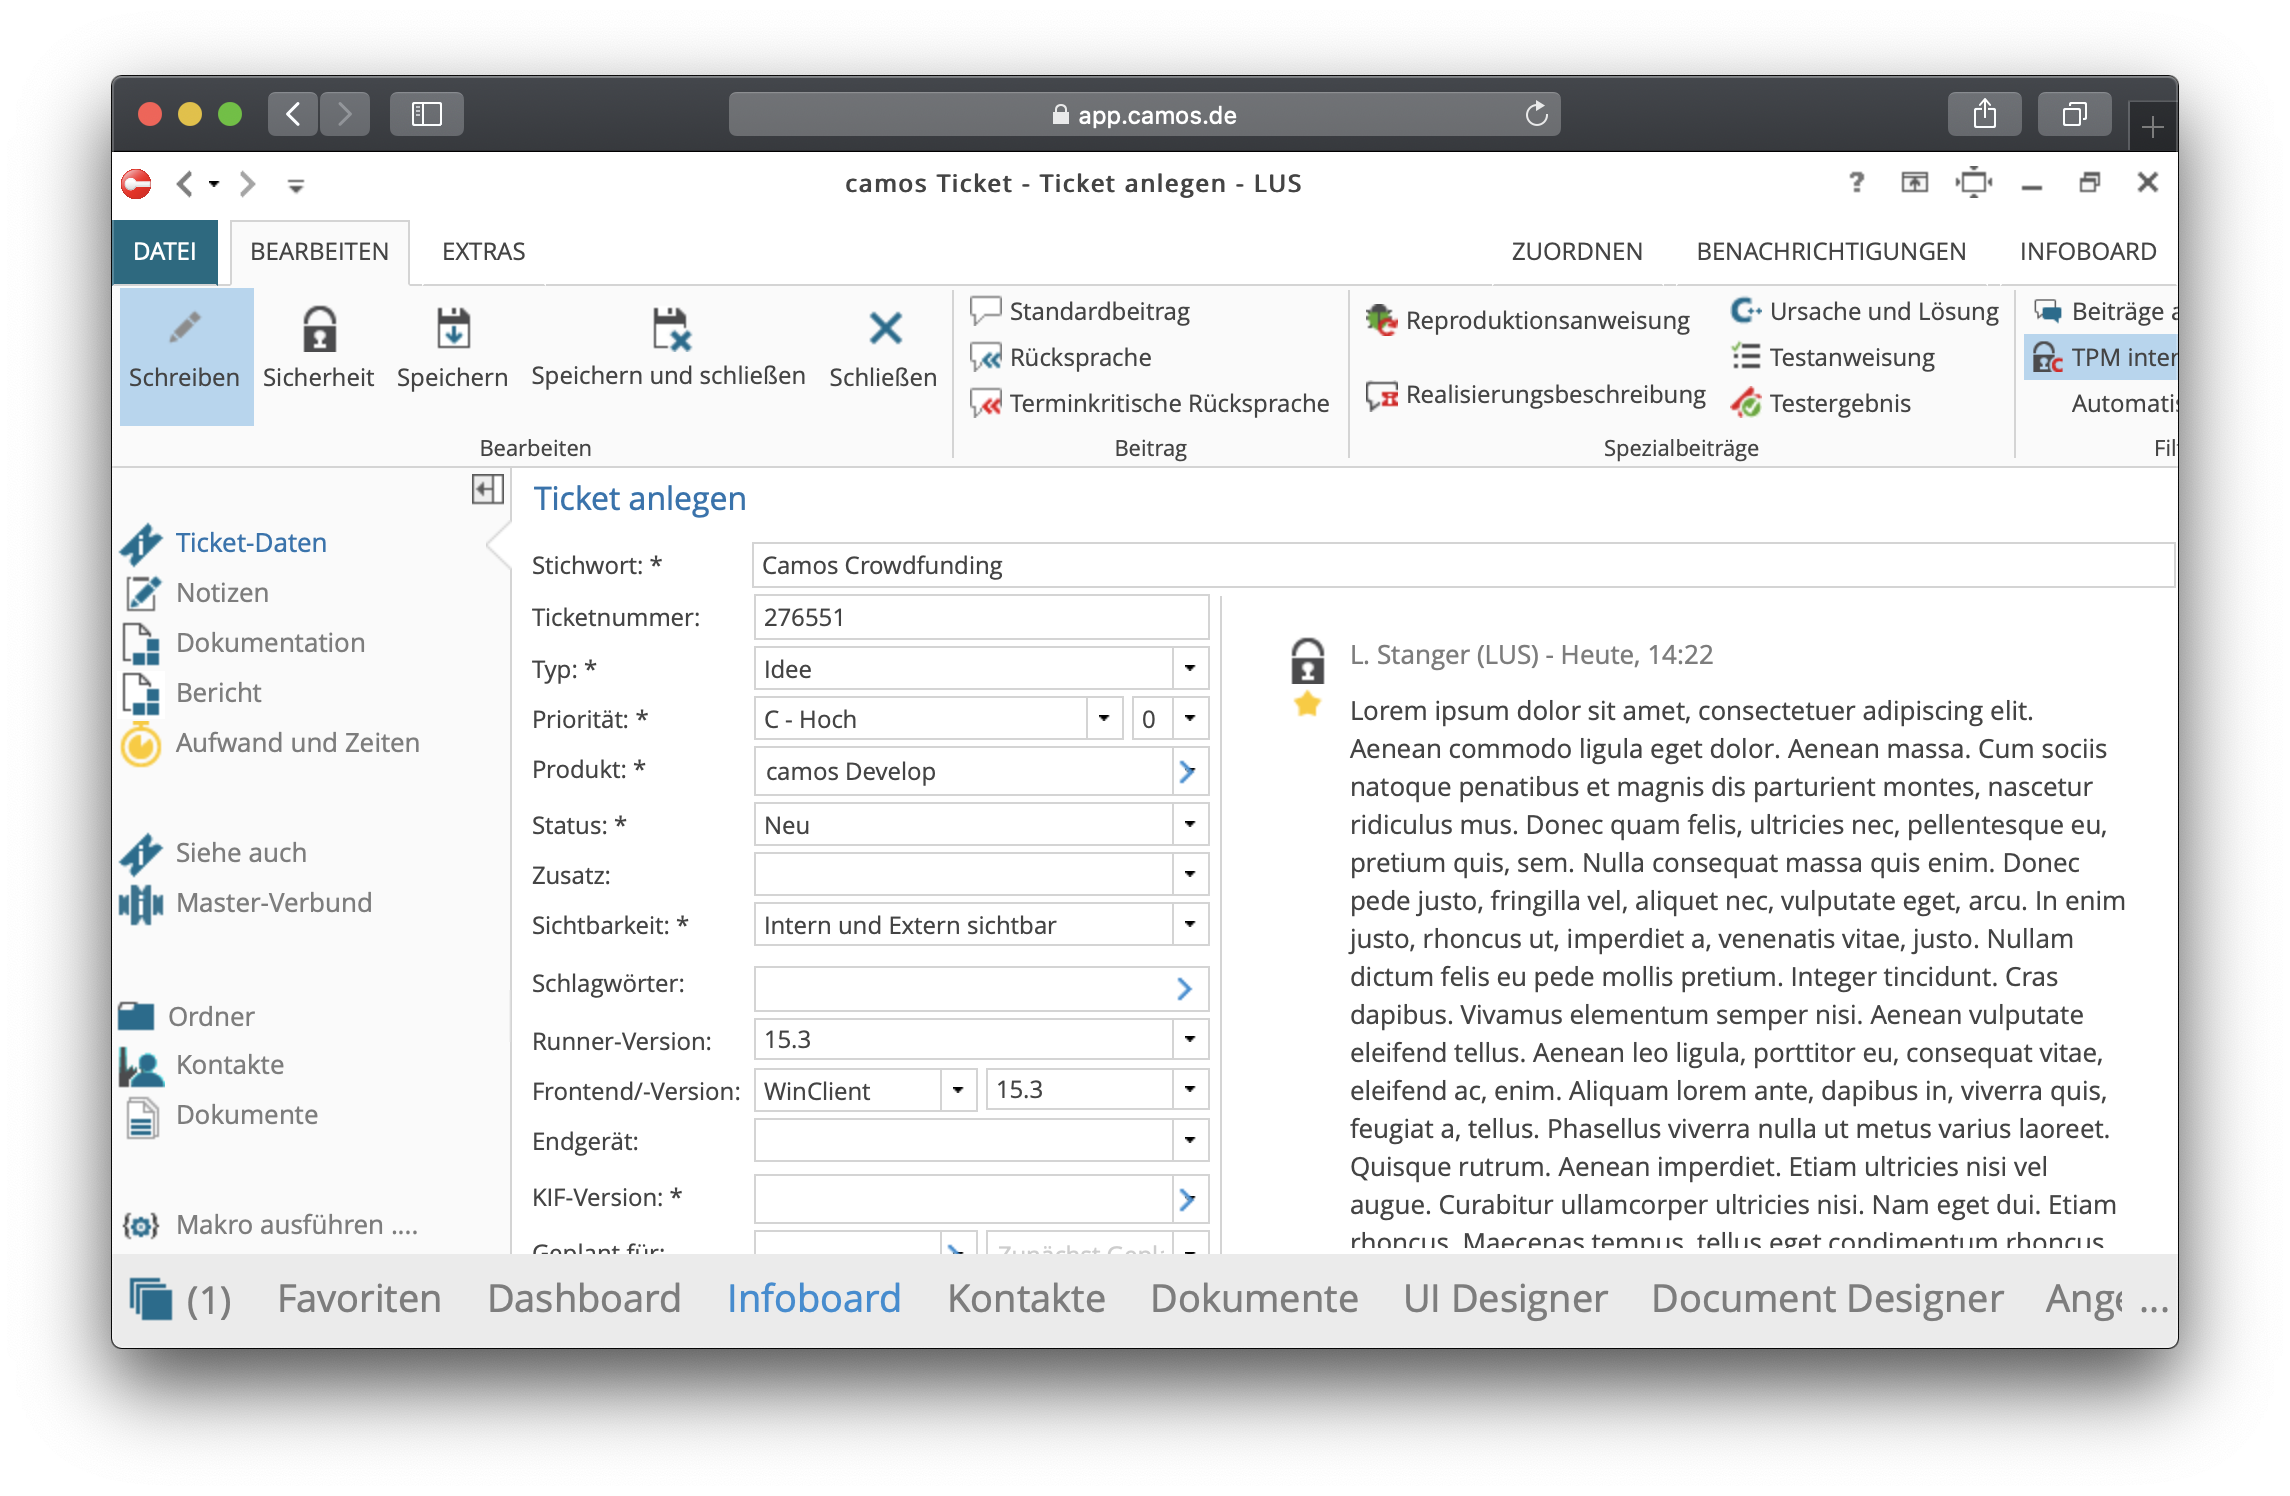
\includegraphics[width=\textwidth]{images/Ticket_erstellen}
	\label{fig:ticket}
	\caption{Benutzeroberfläche zum Erstellen eines Tickets}
\end{figure}

\subsection*{Produktentwicklung Ist-Zustand}
Der Ist-Zustand der Produktentwicklung wurde im Dialog mit einem Mitglied des zugehörigen Entscheidungsgremiums eruiert. Das Gremium bildet sich aus der \ac{GL}, einem \ac{PO} sowie einem erfahrenen Fachexperten und trifft strategische Entscheidungen, wie das Produkt künftig weiterentwickelt wird. Die sich im Ideen-Backlog befindenden Tickets können gleichermaßen von Mitarbeitern sowie Kunden erstellt werden. Der Schlüssel zur Ideen- und Innovationsfindung liegt dabei in der Kommunikation der Dev-Teams, welche ihre täglich gewonnenen Eindrücke aus internen sowie Kunden Projekten in den Prozess einfließen lassen. Als ein weiteres wesentliches Entscheidungskriterium wird die Passgenauigkeit der vorgeschlagenen Idee in die bestehende Strategie gewertet. Die auflaufenden Tickets werden im monatlich abgehaltenen \ac{CPQ}-Gremium diskutiert, bewertet und anschließend in eine Release-Version eingeplant. Sollte es zu einer einstimmigen Ablehnung kommen, wird der Ticketstatus auf abgelehnt gesetzt.

\subsection*{Plattformentwicklung Ist-Zustand}
Im spezifischen wurde der Ist-Zustand in der Plattformentwicklung mit einem Mitglied des dortigen Entscheidungsgremiums erhoben. Im Dialog wurden die Tickets auf die der Plattformentwicklung zugehörigen Produkte beschränkt. Die Abgrenzung wurde hierbei auf die folgenden Produkte vorgenommen:

\begin{itemize}
	\item Laufzeitumgebung camos.Runner
	\item Frontendumgebung camos.WinClient und camos.HTML5Client
	\item Entwicklungsumgebung camos.Develop
	\item Develop-Module camos.LoadBalancer und camos.Scheduler
\end{itemize}

An der Entscheidungsfindung ist, wie zuvor in der Produktentwicklung, ein Gremium beteiligt. Dieses setzt sich aus dem \ac{GL} der Entwicklungsabteilung und den jeweiligen Hauptverantwortlichen der Frontend-, Interpreter- und Plattform-Entwicklung zusammen. Im Rahmen dieses Gremiums werden anhand spezifischer Entscheidungskriterien Tickets aus dem bestehenden Backlog analysiert. Diese Entscheidungskriterien beinhalten einerseits den Fokus auf Großkundenprojekte, andernseits wird versucht, Ideen und Innovationen zur Unterstützung und Weiterentwicklung eines vierteljährlich anstehenden Minor Releases zu erkennen. Tickets, die es nicht in ein kommendes Release geschafft haben, werden stets anhand bestehender Kriterien neu bewertet.

%%Die Umfrage baut sich aus 16 voneinander unabhängigen Fragen auf.
\section{Soll-Zustand}
Für die Aufstellung eines Soll-Zustandes wurde eine firmeninterne Umfrage zum Thema \glqq Möglichkeit und Akzeptanz einer internen Crowdfunding Plattform bei camos\grqq{} durchgeführt. Die daraus erhobenen Erkenntnisse fließen direkt in den Soll-Zustand ein.

\subsection{Aufbau der Umfrage}\label{sec:AufbauUmfrage}
Als Umfragetool wurde sich für die von Google LLC entworfene Lösung Google Forms entschieden. Ausschlaggebend für die Verwendung war die kostenlose Nutzung des Tools sowie die leichte Bedienbarkeit mit weitreichenden Gestaltungsmöglichkeiten der einzelnen Fragen. Die Umfrage setzt sich aus 16 Fragen zusammen, welche initial die bereits vorhandene Kenntnis bezüglich der Themengebiete Crowdfunding und internem Crowdfunding aufnimmt. Weitergehend wird die Akzeptanz und Verwendung des gegenwärtigen Ideen- und Innovationsprozesses examiniert. Dem Umfrageteilnehmer wird im Anschluss die Möglichkeit geboten, Bedenken sowie eigene Interessen im Zusammenhang mit einer internen Crowdfunding Plattform zu nennen. Zuletzt werden Themengebiete erhoben, die mithilfe dieser Plattform behandelt werden sollen. Ziel der Umfrage ist es, die Meinung aller Mitarbeiter, unabhängig ihrer Position zu erfassen und daraus ein auf die Anforderungen angepasstes Konzept zu schaffen. Die Umfrage wird allen beschäftigten Mitarbeitern für einen Monat zur Verfügung gestellt.

%TODO: Umfrage als PDF einfügen.

\subsection{Auswertung der Umfrage}\label{sec:Umfrageauswertung}

Von den befragten 120 Mitarbeitern haben 75 Mitarbeiter an der Umfrage teilgenommen. Um ähnliche Antworten gruppieren zu können, wurde zunächst die Abteilung mit der derzeit ausgeübten Position abgefragt. Als erste themenrelevante Frage wurde der Kenntnisstand des gegenwärtigen Ideen-Einreichungsprozesses abgefragt. Darunter hat sich eine Gruppe von 29 Mitarbeitern (38,7\%) ergeben, die den gegenwärtigen Prozess nicht kennt, wohingegen 46 Mitarbeiter (61,3\%) die Kenntnis am Prozess bejahen. Diese Kennzahl zeigt schon zu Beginn der Umfrage dringenden Handlungsbedarf bezüglich des Ideen- und Innovationsprozess auf. Daraus lässt sich die \ac{NFA}-1 ableiten - \emph{Klare Definition des Ideen- und Innovationsprozesses}. Weitergehend wurde der Kenntnisstand des Auswahlprozesses für neue Ideen abgefragt, welchen 60 Mitarbeiter (80\%) als nicht geläufig bezeichnet haben. Dies bringt \ac{NFA}-2 hervor - \emph{Transparenz des Prozesses zur Entscheidung neuer Ideen und Innovationen}. Da keine Kennzahl zur gegenwärtigen Verwendung des Prozesses vorliegt, wurde diese, unter Verwendung der in Abbildung \ref{fig:frage4} aufgeführten Frage, erhoben. Daraus ist abzuleiten, dass 32 Mitarbeiter (42,7\%) noch nie die Möglichkeit ergriffen haben, eine Idee im Ticketsystem einzustellen. 
\begin{figure}[]
	\centering
	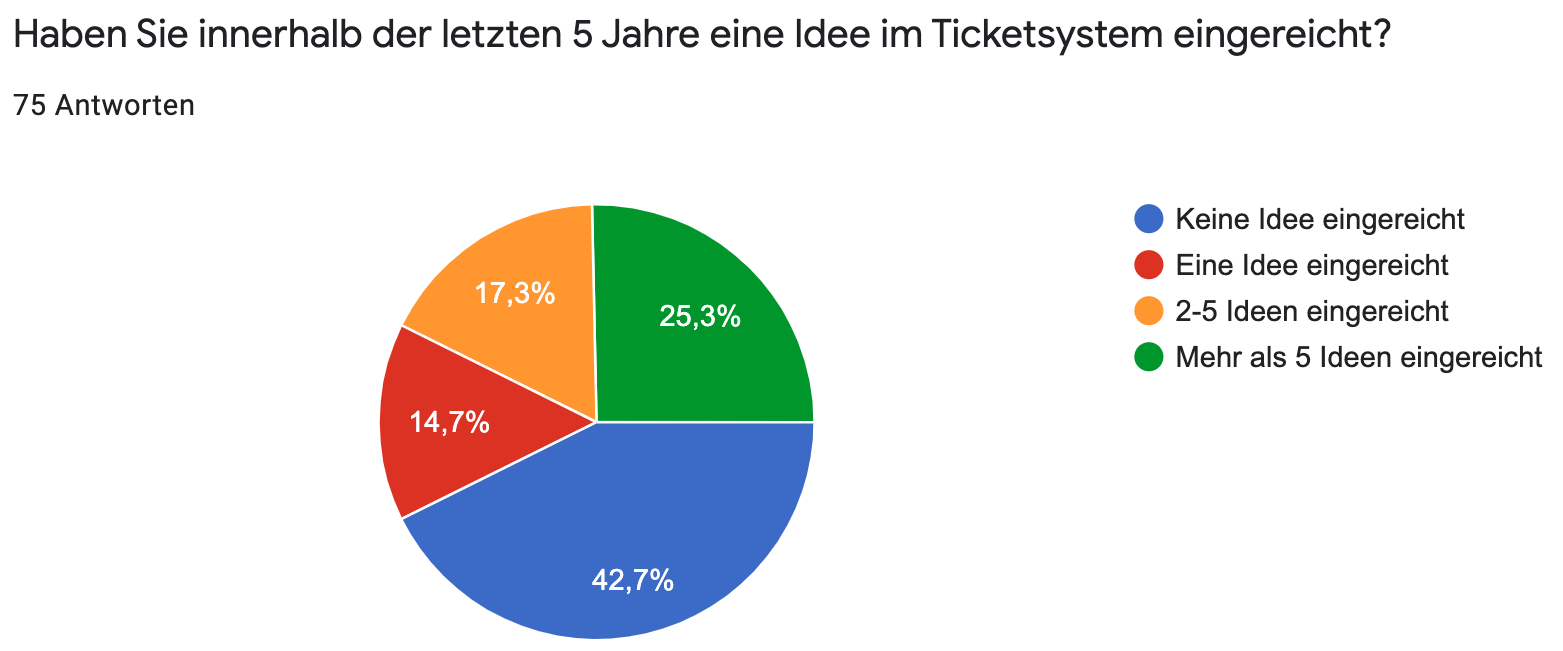
\includegraphics[width=\textwidth]{images/Frage4}
	\caption{Erhebung einer Verwendungskennziffer des gegenwärtigen Prozesses}
	\label{fig:frage4}
\end{figure} 
Durch Auswertung der zuvor angegebenen Abteilung ist zu erkennen, dass die Antwortmöglichkeit \emph{Mehr als 5 Ideen eingereicht} vornehmlich von Mitarbeitern der Beratungs- und Entwicklungsabteilung getroffen wurde. Ein eindeutiger Trend bei der Antwortmöglichkeit \emph{Keine Idee eingereicht} ist in der Abteilungsgruppierung HR/Vertrieb/Verwaltung zu erkennen, was einerseits mit der Fremdheit der Produktpalette zu erklären ist, andererseits hat, wie in Kapitel \ref{sec:internal_crowdfunding} erwähnt, jeder Mitarbeiter ein Potential an Ideen und Innovationen. Da dieses Potential mutmaßlich verloren geht, soll mit Hilfe von \ac{NFA}-3 - \emph{Keine Beschränkung der Ideen und Innovationen auf Produkte} - produktfremden Mitarbeitern eine Möglichkeit der Ideen- und Innovationspublikation geschaffen werden. Von den 43 Mitarbeitern, die innerhalb der letzten fünf Jahre \emph{mindestens} eine Idee eingereicht haben, gaben elf an, dass sie nicht wissen, was mit ihren Ideen passiert. Um dies in einem verbesserten Prozess zu verhindern, soll durch die \ac{FA}-1a - \emph{Benachrichtigung bei Akzeptanz einer Idee} bzw. \ac{FA}-1b - \emph{Benachrichtigung bei Verwerfung einer Idee} mehr Transparenz in den Entscheidungsverlauf gebracht werden. Damit neben dem gegenwärtig verwendeten Prozess die Geläufigkeit des Themas Crowdfunding eingeschätzt werden kann, wurde unter Verwendung einer linearen Skala von 1 - \emph{Ja, ich weiß was der Begriff bedeutet} bis 5 - \emph{Nein, ich weiß nicht was der Begriff bedeutet} eine Kennzahl diesbezüglich eingeholt. Eine kumulierte Anzahl von 11 Mitarbeitern (14,7\%) haben hierbei eine \glqq{}3\grqq{} oder schlechter vergeben. Folglich sollte eine Erläuterung des Begriffs \emph{Crowdfunding} stattfinden, um die Zahl der Mitarbeiter zu minimieren. Zusätzlich zu dieser Erläuterung sollte der Unterschied zwischen Crowdfunding und internem Crowdfunding geklärt werden, da die überwiegende Mehrheit (76\%) angegeben hat, keine Kenntnisse bezüglich des internen Crowdfundings zu besitzen. Dessen ungeachtet ist die Akzeptanz an eine interne Crowdfunding Plattform und die damit einhergehende Modifikation des gegenwärtigen Prozesses mit 62 Ja-Stimmen (82,7\%) deutlich vorhanden. 
\begin{figure}[t]
	\centering
	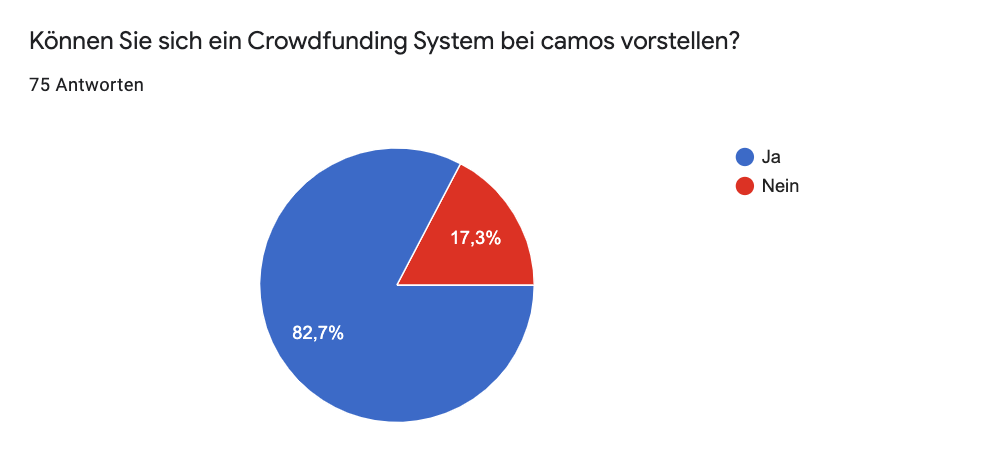
\includegraphics[width=\textwidth]{images/Frage9}
	\caption{Validierung der Akzeptanz einer Prozessänderung}
	\label{fig:frage9}
\end{figure} 
Mit ein Grund hierfür ist das Resultat der in Abbildung \ref{fig:frage7} aufgeführten Frage. Hieraus lässt sich erkennen, dass lediglich 10 Mitarbeiter (13,3\%) der Ansicht sind, dass die besten Ideen den Weg in das Produkt finden. Auf der anderen Seite jedoch, wurde von 26 Mitarbeitern (34,7\%) die Ansicht geäußert, dass gute Ideen teilweise nicht wahrgenommen werden. Die von über einem Drittel der Umfrageteilnehmer getroffene Aussage, dass der gegenwärtige Prozess gute Ideen teilweise nicht wahrnimmt, unterschreibt erneut die Dringlichkeit einer Prozessüberarbeitung. Auf die Frage, ob bereits eine Ticketidee des Umfrageteilnehmers für ein internes Crowdfunding System vorhanden ist, hatten nur 19 Mitarbeiter (25,3\%) mit \glqq{}Ja\grqq{} abgestimmt. 
\begin{figure}[b]
	\centering
	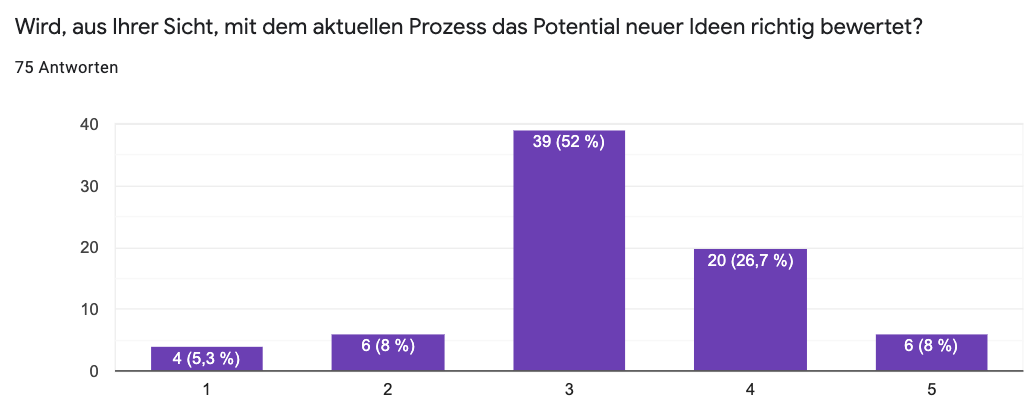
\includegraphics[width=\textwidth]{images/Frage7}
	\caption{Gegenwärtige Ansicht bezüglich des Entscheidungsprozesses}
	\label{fig:frage7}
\end{figure} 
In Kombination mit der Frage, ob ein Belohnungssystem für erfolgreich umgesetzte Ideen eingeführt werden sollte, welche die Mehrzahl der Mitarbeiter (60\%) bejaht haben, lässt sich durch \ac{FA}-2 - \emph{Belohnungssystem} ein Stimulus bezüglich der zukünftigen Teilnahmequote setzen. Um darüber hinaus funktionale sowie nicht-funktionale Aspekte der zukünftigen Lösung erheben zu können, wurden mithilfe einer Multiple-Choice Umfrage zunächst vorgegebene Aspekte der Bewertung unterzogen. Dabei wurden die vorgegebenen Aspekte grundlegend als Positiv bewertet. Aufgrund der positiven Resonanz resultieren \ac{FA}-3 - \emph{Mobile Erreichbarkeit der Plattform} sowie \ac{FA}-4 - \emph{Keine quantitative Begrenzung der Ideenerstellung}. Weitergehend wird die Zusammenführung von Ideentickets, welche den gleichen Inhalt beschreiben, gefordert. Dies soll durch \ac{FA}-5 - \emph{Zusammenführung von Tickets} gewährleistet werden. Als ein weiterer maßgeblicher Aspekt wurde die Filtermöglichkeit von Ideentickets bewertet, um interessante Tickets für den Anwender einfacher auffindbar zu machen. Um die Umsetzung dieses Aspekts sicherzustellen, wird \ac{FA}-6 - \emph{Filtermöglichkeit von Ideentickets} aufgestellt. Als wichtigster Aspekt wurde, seitens der Umfrageteilnehmer, die gleichwertige Gewichtung von Stimmabgaben, unabhängig der Position des Mitarbeiters, gewählt. Dies soll mithilfe von \ac{NFA}-4 - \emph{Gleichwertige Gewichtung der Stimmen} sichergestellt werden. Über die Bewertung der vorgegebenen Aspekte hinaus, haben sich weitere Faktoren ergeben, die den Umfrageteilnehmern wichtig sind. Diese wurden durch die Möglichkeit einer Freitext Eingabe erhoben, woraus sich \ac{FA}-7 - \emph{Feedback über Status einer Idee}, \ac{FA}-8 - \emph{Möglichkeit der Kommentierung einer Idee}, \ac{FA}-9 - \emph{Sichtbarkeit der Stimmen} - sowie \ac{FA}-10 - \emph{Anonyme Abstimmungsmöglichkeit} ergeben. Abschließend wurde der Umgang mit älteren und noch nicht realisierten Ideentickets erfasst, welcher von 44 Mitarbeitern (62,9\%) mit \emph{Das Ziel wurde nicht erreicht. Für eine zweite Chance muss die Idee reaktiviert werden} - abgestimmt wurde. Daraus entsteht \ac{NFA}-5 - \emph{Abgelaufene Ideentickets müssen reaktiviert werden}.
\begin{figure}[hb]
	\centering
	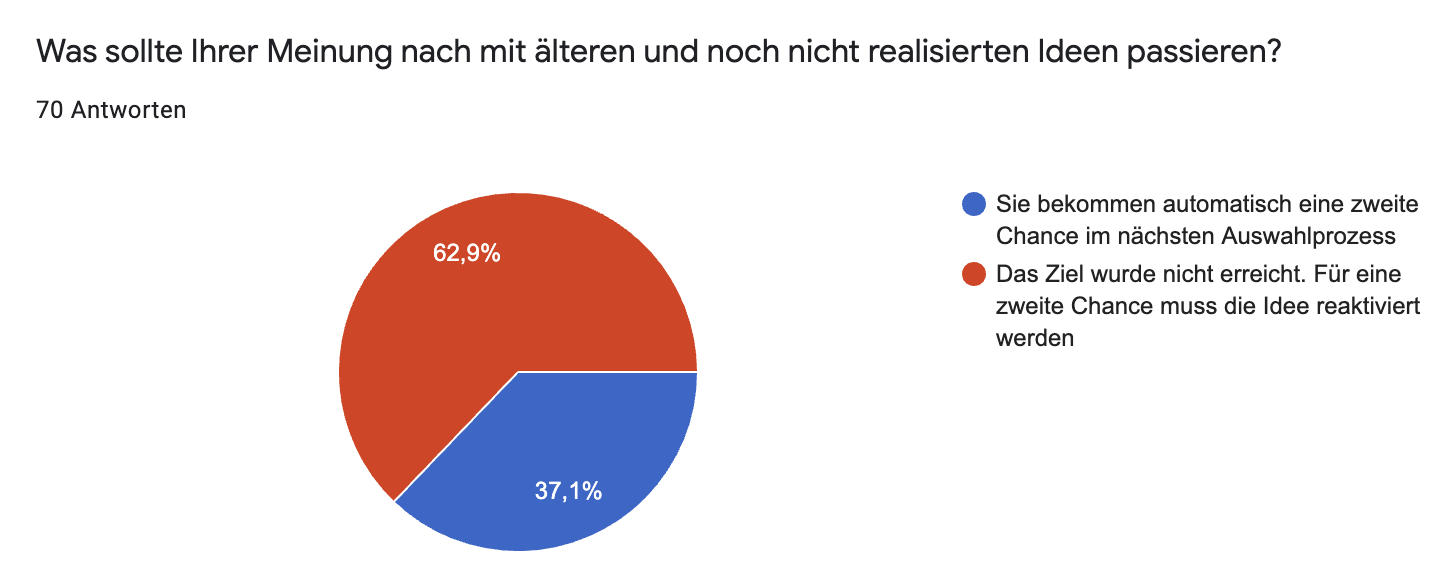
\includegraphics[width=\textwidth]{images/Frage16}
	\caption{Umfrageergebnis der Handhabung abgelaufener Ideentickets}
	\label{fig:frage16}
\end{figure} 
\newpage
\subsection{Tabellarische Aufstellung der erhobenen Anforderungen}\label{sec:anforderungen_tabellarisch}

\begin{longtable}[h]{|l|p{10cm}|}
\hline
Anforderungskennzeichen & Anforderungskurzbeschreibung \\
\hline
FA-1\label{itm:FA-1} & Als Anwender möchte ich bei Akzeptanz einer Idee informiert werden.\\
\hline
FA-2 & Als Anwender möchte ich für konstruktive Ideen belohnt werden.\\
\hline
FA-3 & Als Anwender möchte ich die Crowdfunding Plattform mobil erreichen können.\\
\hline
FA-4 & Als Anwender möchte ich nicht durch eine quantitative Einschränkung der Ideen begrenzt werden.\\
\hline
FA-5 & Als Anwender möchte ich Ideentickets mit ähnlichem Inhalt zusammenführen können.\\
\hline
FA-6 & Als Anwender möchte ich ausgiebige Filtermöglichkeiten erhalten, um Tickets meines Interessengebiets leichter ausfindig zu machen.\\
\hline
FA-7 & Als Anwender möchte ich Feedback über den Status einer Idee erhalten.\\
\hline
FA-8 & Als Anwender möchte ich für mich relevante Ideen kommentieren können.\\
\hline
FA-9 & Als Anwender möchte ich stets die Anzahl der Stimmen einsehen können, die eine Idee unterstützen.\\
\hline
FA-10 & Als Anwender möchte ich die Möglichkeit haben, Ideen anonym unterstützen zu können.\\
\hline
NFA-1 & Der Ideen- und Innovationsprozess muss klar definiert sein.\\
\hline
NFA-2 & Der Entscheidungsprozess von Ideen und Innovationen muss transparent einsehbar sein.\\
\hline
NFA-3 & Ideen und Innovationen dürfen nicht auf Produktebene beschränkt werden.\\
\hline
NFA-4 & Stimmabgaben müssen zu jeder Zeit, unabhängig der Position des Mitarbeiters, gleich gewichtet werden. \\
\hline
NFA-5 & Wird ein Ticket in einer vorbestimmten Zeit nicht umgesetzt muss es vom Ersteller reaktiviert werden. \\
\hline
\caption{Tabellarische Auflistung funktionaler und nicht funktionaler Anforderungen}\label{tab:Anforderungsanalyse}
\end{longtable}











